%\setcounter{section}{30}
\section{ĐỊNH NGHĨA VÀ Ý NGHĨA CỦA ĐẠO HÀM}
\subsection{KIẾN THỨC CẦN NHỚ}
\subsubsection{Định nghĩa đạo hàm tại một điểm}
\begin{enumerate}[\iconMT]
	\item \indam{Định nghĩa:} Cho hàm số $y=f(x)$ xác định trên $(a;b)$ và $x_0 \in (a;b)$. Xét giới hạn $\lim\limits_{x\to x_0}\dfrac{f(x)-f(x_0)}{x-x_0}$ $\quad (1)$. Nếu giới hạn (1)  \textbf{hữu hạn} thì kết quả đó được gọi là đạo hàm của hàm số $y=f(x)$ tại điểm $x_0$. Kí hiệu $f'(x_0)$ hay $y'(x_0)$. Tức là
		\boxmini{$f'(x_0)=\lim\limits_{x\to x_0}\dfrac{f(x)-f(x_0)}{x-x_0}$  $\quad (2)$}
	\item \indam{ Lưu ý:}
	\begin{itemize}
		\item Đại lượng $\Delta x =x-x_0$ được gọi là số gia của biến tại $x_0$.
		\item Đại lượng$\Delta y =f(x)-f(x_0)=f(x_0+\Delta x)-f(x_0)$ được gọi là số gia tương ứng của hàm số.
	\end{itemize}
	Khi đó công thức (2) được viết thành 
		\boxmini{$f'(x_0)=\lim\limits_{\Delta x \to 0}\dfrac{\Delta y}{\Delta x}$ $\quad (3)$} 
	\begin{note}
		Muốn tính đạo hàm tại một điểm cho trước, ta chọn một trong hai công thức (2) hoặc (3).
	\end{note}
\end{enumerate}

\subsubsection{Đạo hàm trên một khoảng}
Hàm số $y=f(x)$ được gọi là có đạo hàm trên khoảng $(a;b)$ nếu nó có đạo hàm tại mọi điểm  $x$ trên khoảng đó. Kí hiệu $y'$ hoặc $f'(x)$

\subsubsection{Ý nghĩa vật lý của đạo hàm}
\begin{itemize}
	\item [\iconMT] \indam{Vận tốc tức thời:}  Xét chuyển động thẳng xác định bởi phương trình $s=f\left( t \right)$, với $f\left( t \right)$ là hàm số có đạo hàm. Khi đó, vận tốc tức thời của chất điểm tại thời điểm $t_0$ là đạo hàm của hàm số $s=f\left( t \right)$ tại $t_0$. Nghĩa là
	$$v\left( t_0 \right)=s'\left(t_0 \right)=f'\left(t_0 \right).$$
	\item [\iconMT] \indam{Cường độ tức thời:} Điện lượng $Q$ truyền trong dây dẫn xác định bởi phương trình $Q=f\left( t \right)$, với $f\left( t \right)$ là hàm số có đạo hàm. Khi đó, cường độ tức thời của dòng điện tại thời điểm $t_0$ là đạo hàm của hàm số $Q=f\left( t \right)$ tại $t_0$. Nghĩa là 
	$I\left( t_0 \right)=Q'\left( t_0 \right)=f'\left( t_0 \right).$
\end{itemize}

\subsubsection{Ý nghĩa hình học của đạo hàm}
\immini{Cho hàm số $y=f(x)$ xác định trên $(a;b)$ và có đạo hàm tại $x_0 \in (a;b)$. Gọi $\mathscr{(C)}$ là đồ thị của hàm số đó. Ta có hai kết quả sau:
\begin{gachsoc}
	\begin{itemize}
		\item [\ding{172}] $f'(x_0)$ là hệ số góc của tiếp tuyến $\Delta$ của đồ thị $\mathscr{(C)}$ tại điểm $M(x_0;y_0)$.
		\item [\ding{173}] Phương trình tiếp tuyến $\Delta \colon y-y_0=f'(x_0)(x-x_0)$.
		\begin{itemize}
			\item $(x_0;y_0)$ là tọa độ tiếp điểm;
			\item $f'(x_0)$ là hệ số góc của tiếp tuyến.
		\end{itemize}
	\end{itemize}
\end{gachsoc}}{
	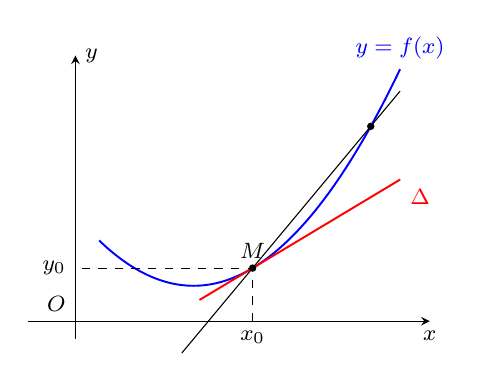
\begin{tikzpicture}[smooth,samples=300,scale=0.75,y=0.6cm,>=stealth,font=\footnotesize]
	\draw[->] (-0.8,0)--(6,0) node[below]{$x$};
	\draw[->] (0,-0.5)--(0,7.5) node[right]{$y$};
	\draw (0,0) node[above left]{$O$};
	\draw[line width=0.7pt,domain=0.4:5.5,blue] plot(\x,{0.5*(\x-2)^2+1})node[above]{$y=f(x)$};
	\draw[line width=0.4pt,domain=1.8:5.5] plot(\x,{2*(\x)-4.5});
	\draw[line width=0.7pt,domain=2.1:5.5,red] plot(\x,{(\x)-1.5})node[below right]{$\Delta$};
	\draw[fill=black] (3,1.5) circle(1.5pt) (5,5.5) circle(1.5pt);
	\draw[dashed] (3,0)node[below]{$x_0$}--(3,1.5)node[above]{$M$}--(0,1.5)node[left]{$y_0$};
	%\node[right] at (2,2.4) {$2$};
	\end{tikzpicture}}

\subsubsection{Quan hệ giữa sự tồn tại đạo hàm và tính liên tục}
\begin{itemize}
	\item [\iconMT] \indam{Định lý:} Nếu hàm số  $y=f(x)$  có đạo hàm tại điểm $x_0$   thì nó liên tục tại điểm đó.
	\item [\iconMT] \indam{Chú ý: }
	\begin{gachsoc}
		\begin{itemize}
			\item [$\bullet$] Chiều đảo lại \textbf{không đúng}. Tức là, hàm số liên tục tại $x_0$ có thể không có đạo hàm tại $x_0$.
			\item [$\bullet$] Hàm số không liên tục tại $x_0$ thì không có đạo hàm tại điểm đó.
		\end{itemize}
	\end{gachsoc}
\end{itemize}
